\documentclass[../PianoDiProgetto.tex]{subfiles}
\begin{document}
	\section{Pianificazione}
	Date le scadenze riportate nella sottosezione 1.5, si è deciso di suddividere lo sviluppo del propgetto in cinque macro-periodi di lavoro:
	\begin{itemize}
		\item \textbf{Analisi};
		\item \textbf{Analisi di dettaglio};
		\item \textbf{Progettazione architetturale};
		\item \textbf{Progettazione di dettaglio e Codifica};
		\item \textbf{Validazione};
	\end{itemize}
	Ogni periodo è stato poi suddiviso in varie attività, alle quali sono state associate una o
	più risorse. Le attività designate sono state poi a loro volta scomposte in sotto-attività
	ancor più di dettaglio. \\
	Delle sotto-attività è stato riportato unicamente il Gantt così da evidenziare la piani-
	ficazione di dettaglio ma restando focalizzati sui concetti di maggiore importanza.
	

		\subsection{Analisi}
		\textbf{Periodo} : Da 27/02/2017 a 25/03/2017. \\
		Questo periodo comincia con la formazione del gruppo di lavoro e prosegue fino alla scadenza di consegna dei documenti necessari alla \revisionedeirequisiti.
		\begin{itemize}
			\item \textbf{Norme di progetto}: l'\amministratore\ si consulta con i membri del gruppo e definisce le norme che saranno seguite durante l'attuazione di tutte le attività di progetto. In base alle direttive da lui emanate viene redatto il documento \normediprogetto; Il rispetto di tali norme sarà poi certificato dai \verificatori. Questa attività è anticipata rispetto alle altre poiché ne regola direttamente lo svolgimento;
			\item \textbf{Piano di qualifica}: vengono definiti gli obiettivi e le metodologie che ogni membro del gruppo
			\kaleidoscode\ adotterà per garantire un determinato livello di qualità del prodotto; in particolare, vengono individuate tutte le strategie di verifica e validazione degli artefatti prodotti e dei processi attuati. Viene redatto il \pianodiqualifica;
			\item \textbf{Studio di fattibilità}: vengono valutati singolarmente tutti i capitolati e viene redatto uno \studiodifattibilita. Viene studiata la complessità delle varie proposte mediante l’abbozzo di Analisi dei Requisiti ad alto livello. Al termine dello studio si sceglie il capitolato da sviluppare;
			
			\item \textbf{Analisi dei requisiti}: viene approfondita l'analisi di base svolta nell'ambito dello \studiodifattibilita\ e si inizia la redazione del documento \analisideirequisiti, il quale verrà continuamente integrato fino a poco prima della data di consegna. Si inizia analizzando i requisiti obbligatori, da quelli più generali procedendo verso quelli di un livello maggiore  di dettaglio;  verrà organizzato un sufficiente numero di incontri con il proponente al fine di consolidare i requisiti individuati fino a quel momento; dopo ogni incontro, l'\analisideirequisiti\ viene integrata con i requisiti e casi d'uso che sono stati consolidati con il proponente, dopodiché si procede con l'individuazione e l'analisi di ulteriori requisiti e casi d'uso da sottoporre alla valutazione del proponente;
		
			\item \textbf{Piano di progetto}: sulla base delle scadenze e del modello di sviluppo adottato, il \responsabilediprogetto\ definisce una prima pianificazione così da regolare le attività di gruppo; stima le risorse, costi e tempi necessari a svolgere i periodi di progetto; inoltre, individua i rischi nei quali il gruppo \kaleidoscode\ potrebbe incorrere, definendo politiche di mitigazione per essi. Da tale studio, il \responsabilediprogetto\ redige una prima stesura del \pianodiprogetto;
			
			\item \textbf{Glossario}: contestualmente alla redazione degli altri documenti viene compilato un glossario che contenga la spiegazione dei termini considerati di non immediata comprensione. Tale documento viene incrementato dai redattori dei documenti ad ogni aggiunta di termini che necessitano di spiegazione;
			

		\end{itemize}
		% DIAGRAMMA DI GANTT DELLE ATTIVITÀ
		\begin{figure}[H]
			\centering
			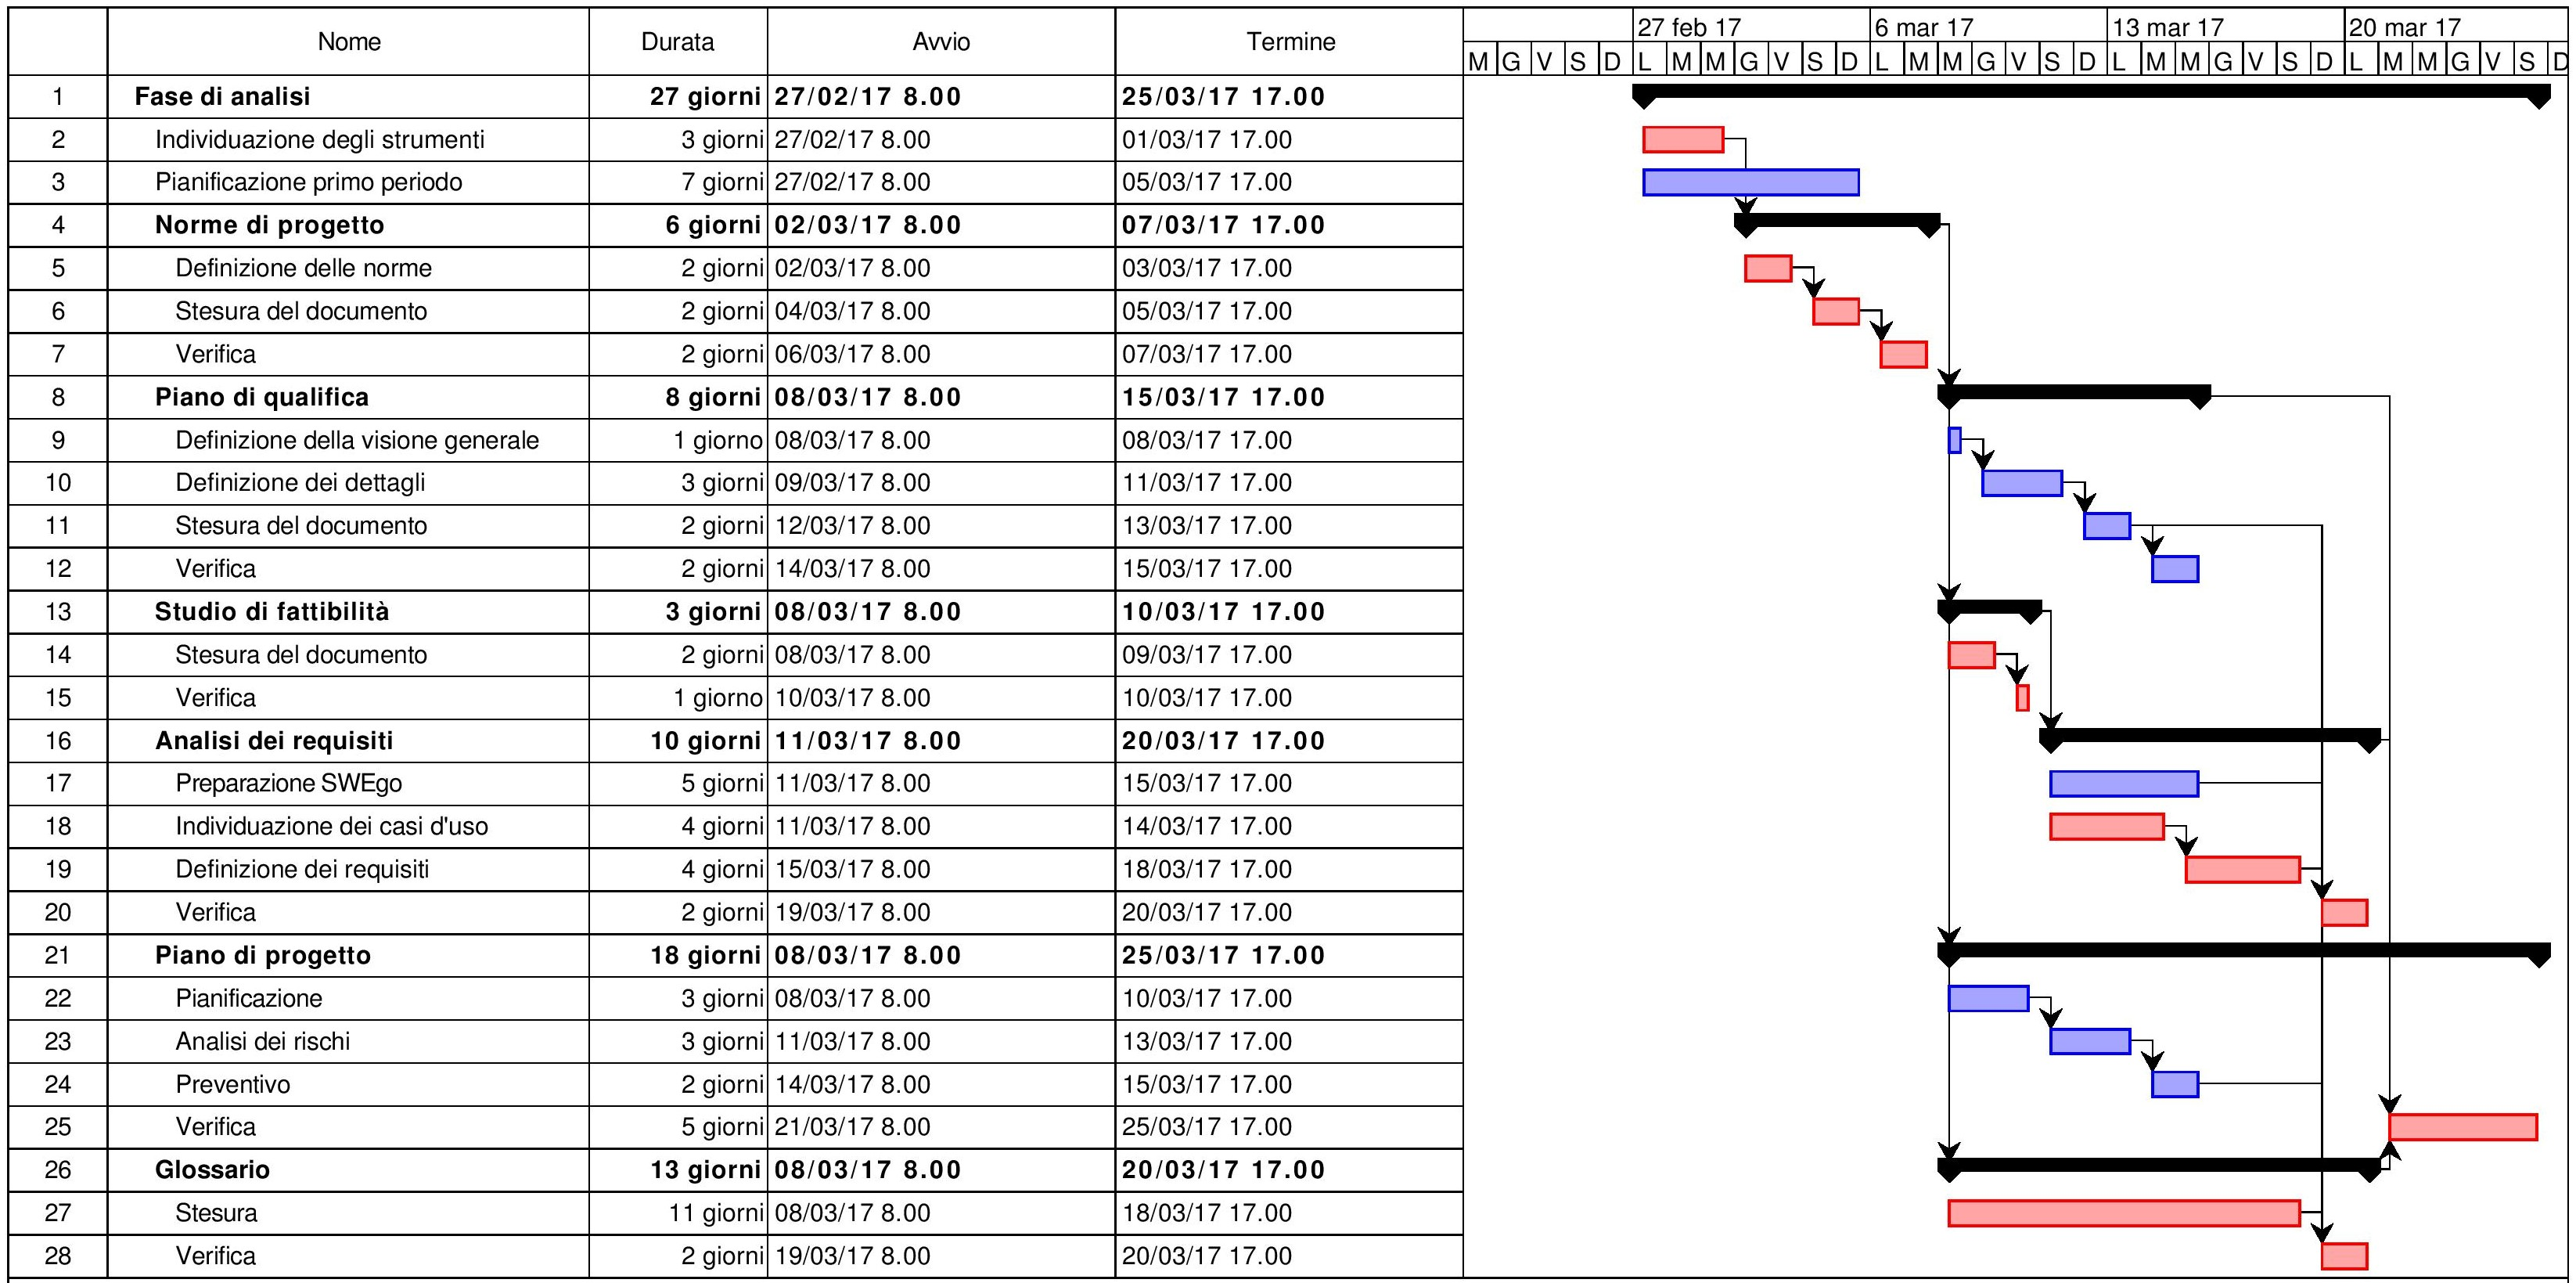
\includegraphics[scale=0.55]{Figures/Gantt_Analisi.jpg}
			\caption{Analisi: Diagramma di Gantt}
		\end{figure}
			
			
			
		\subsection{Analisi di dettaglio}
		\textbf{Periodo} : Da 26/03/2017 a 03/04/2017. \\
		Questo periodo inizia con la fine del periodo di Analisi e prosegue fino alla data di scadenza della consegna della \revisionedeirequisiti. \\
		In questo periodo vengono consolidati i requisiti richiesti dal sistema e vengono analizzati i requisiti di maggior dettaglio, i requisiti desiderabili e quelli opzionali; 
		\begin{itemize}
			\item \textbf{Analisi di dettaglio}: si approfondisce quanto svolto in sede di analisi e vengono consolidati i requisiti richiesti dal sistema. Inoltre, vengono analizzati i requisiti di maggior dettaglio, i requisiti desiderabili e quelli opzionali; i requisiti prodotti da tale analisi, una volta consolidati, vengono integrati nel documento \analisideirequisiti;
			\item \textbf{Incremento e Verifica}: se necessario vengono aggiornati e verificati i documenti redatti in precedenza. In particolare, vengono riportati il consuntivo di periodo e il riscontro avuto fino a quel momento dei rischi analizzati, nel \pianodiprogetto. \\ Inoltre, viene specificata una lista di controllo degli errori più comuni riscontrati dai \verificatori\ e vengono riportati i resoconti delle attività di verifica effettuate.
		\end{itemize}
		% DIAGRAMMA DI GANTT DELLE ATTIVITÀ
		\begin{figure}[H]
			\centering
			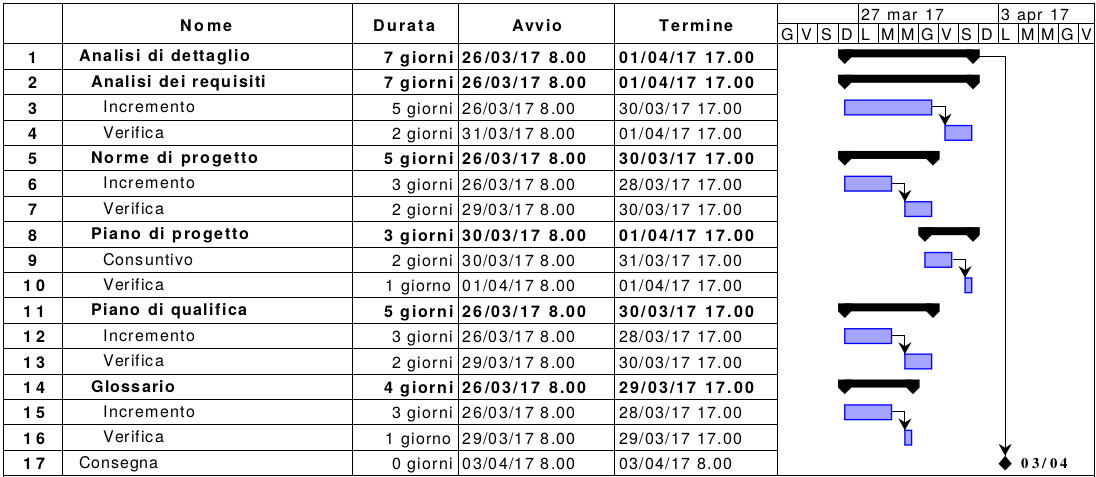
\includegraphics[scale=0.55]{Figures/Gantt_AnalisiDettaglio.jpg}
			\caption{Analisi di dettaglio: Diagramma di Gantt}
		\end{figure}
	
	
	
		\subsection{Progettazione architetturale}
		\textbf{Periodo} : Da 04/04/2017 a 27/04/2017. \\
		Questo periodo comincia al termine del periodo di Analisi di dettaglio e termina con la consegna dei documenti per la \revisionediprogettazione.
		\begin{itemize}
			\item \textbf{Specifica Tecnica}: dopo un primo periodo di auto formazione necessaria alla successiva progettazione ad alto livello del sistema, i \progettisti\ definiscono un'architettura generale del sistema, individuando le componenti di più alto livello. Inoltre, vengono specificati i design pattern utilizzati nella definizione della architettura. I risultati di tale attività vengono documentati nella \specificatecnica, redatta dal \progettista. \\
			Una volta identificato un discreto numero di componenti dell'architettura generale, verrà definito un incontro con il proponente al fine di consolidare le componenti individuate; tale attività si ripete fino ad ottenere un'architettura generale, ma sufficientemente completa a tracciare i requisiti di alto livello con le componenti individuate.

			\item \textbf{Incremento e Verifica}: se necessario vengono aggiornati e verificati i documenti redatti in precedenza, secondo le indicazioni riportate nella valutazione della \revisionedeirequisiti. \\ Vengono riportati il consuntivo di periodo, il preventivo a finire e il riscontro avuto fino a quel momento dei rischi analizzati, nel \pianodiprogetto. \\  Inoltre, viene incrementata la lista di controllo degli errori più comuni riscontrati dai \verificatori\ e vengono riportati i resoconti delle attività di verifica effettuate. \\
			
		\end{itemize}
		% DIAGRAMMA DI GANTT DELLE ATTIVITÀ
		\begin{figure}[H]
			\centering
			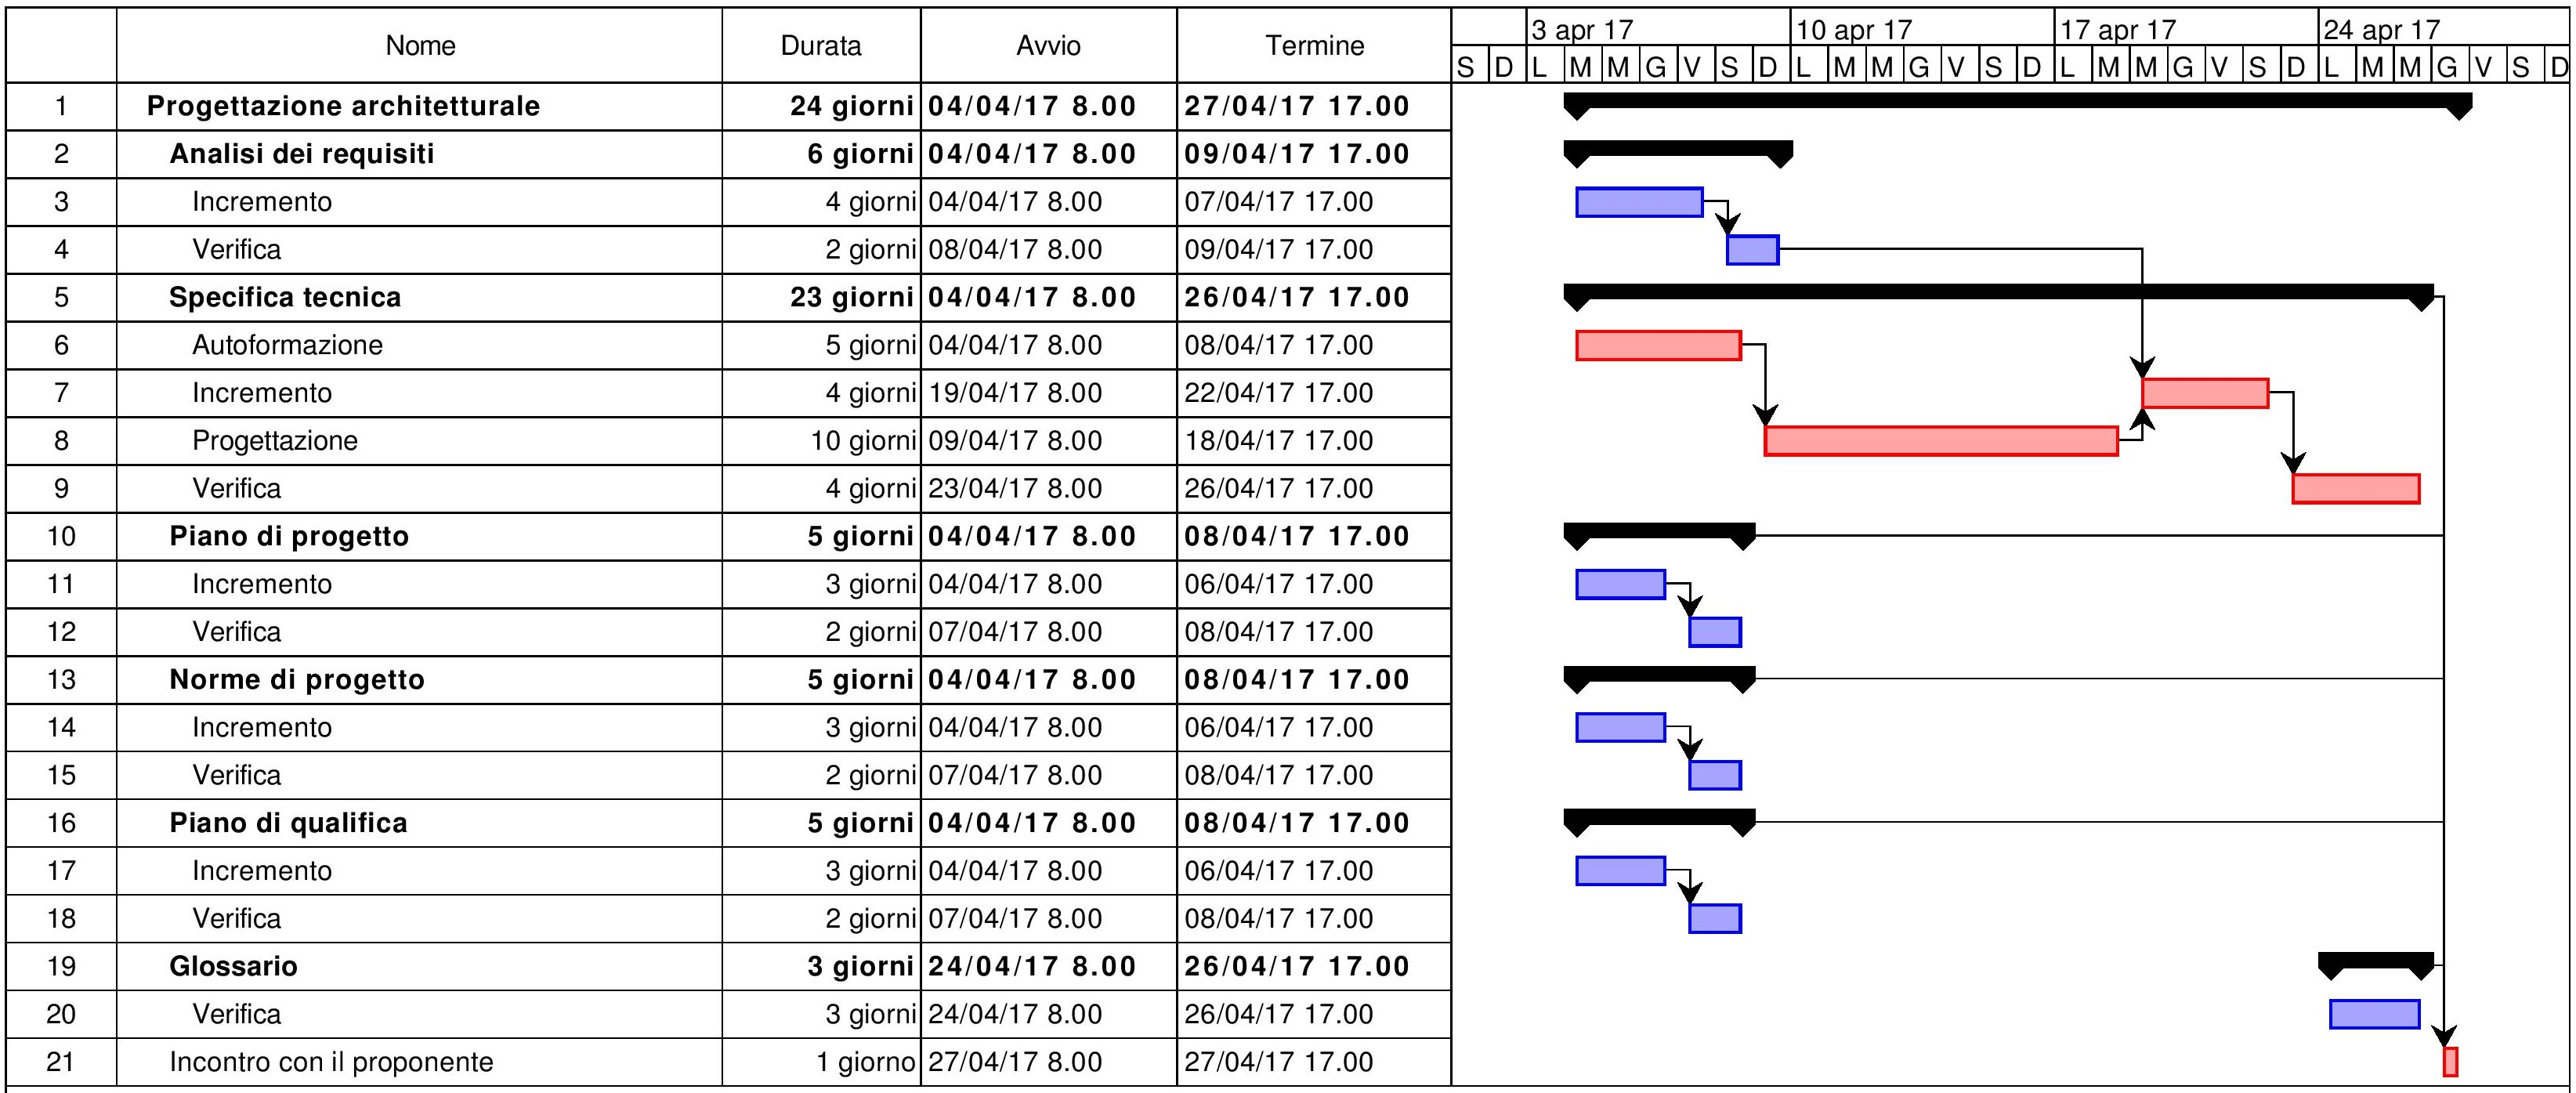
\includegraphics[scale=0.55]{Figures/Gantt_ProgettazioneArchitetturale}
			\caption{Progettazione architetturale: Diagramma di Gantt}
		\end{figure}
		
		
		
		\subsection{Progettazione di dettaglio e Codifica}
		\textbf{Periodo} : Da 28/04/2017 a 20/06/2017. \\
		Questo macro-periodo comincia al termine del periodo di Progettazione architetturale e prosegue fino alla scadenza della consegna della \revisionediqualifica.
		È a sua volta divisa in 3 grandi iterazioni che riguardano Progettazione di dettaglio e Codifica rispettivamente dei requisiti obbligatori, desiderabili e opzionali.
		\begin{itemize}
			\item \textbf{Definizione di prodotto}: si definiscono approfonditamente la struttura e le relazioni dei vari componenti del prodotto, in accordo con quanto descritto nella \specificatecnica. In base a questi viene redatta la \definizionediprodotto;
			\item \textbf{Codifica}: inizia in questo periodo lo sviluppo del codice del prodotto, seguendo la struttura stabilita dalla \definizionediprodotto. Una volta sviluppate e integrate un certo numero di componenti che implementano funzionalità 'tangibili' del prodotto, queste vengono sottoposte alla valutazione del proponente e integrate nel documento \definizionediprodotto. In questo modo il prodotto viene costruito in maniera incrementale e si hanno continui feedback da parte del proponente;
			\item \textbf{Manuale Utente e Manuale Amministratore}: contestualmente alla progettazione di dettaglio del prodotto si redigono i manuali contenenti le linee guida per l'utilizzo del prodotto; 
			\item \textbf{Incremento e Verifica}: se necessario vengono aggiornati e verificati i documenti redatti in precedenza, secondo le indicazioni riportate nella valutazione della \revisionediprogettazione. \\
			I \progettisti\ incrementano la progettazione del sistema definendo le componenti di dettaglio atte a soddisfare tutti i requisiti obbligatori e, successivamente, quelli desiderabili. \\
			 Vengono riportati il consuntivo di periodo, il preventivo a finire e il riscontro avuto fino a quel momento dei rischi analizzati, nel \pianodiprogetto. \\  Inoltre, viene incrementata la lista di controllo degli errori più comuni riscontrati dai \verificatori\ e vengono riportati i resoconti delle attività di verifica effettuate.  
		\end{itemize}
		% DIAGRAMMA DI GANTT DELLE ATTIVITÀ
		\begin{figure}[H]
			\centering
			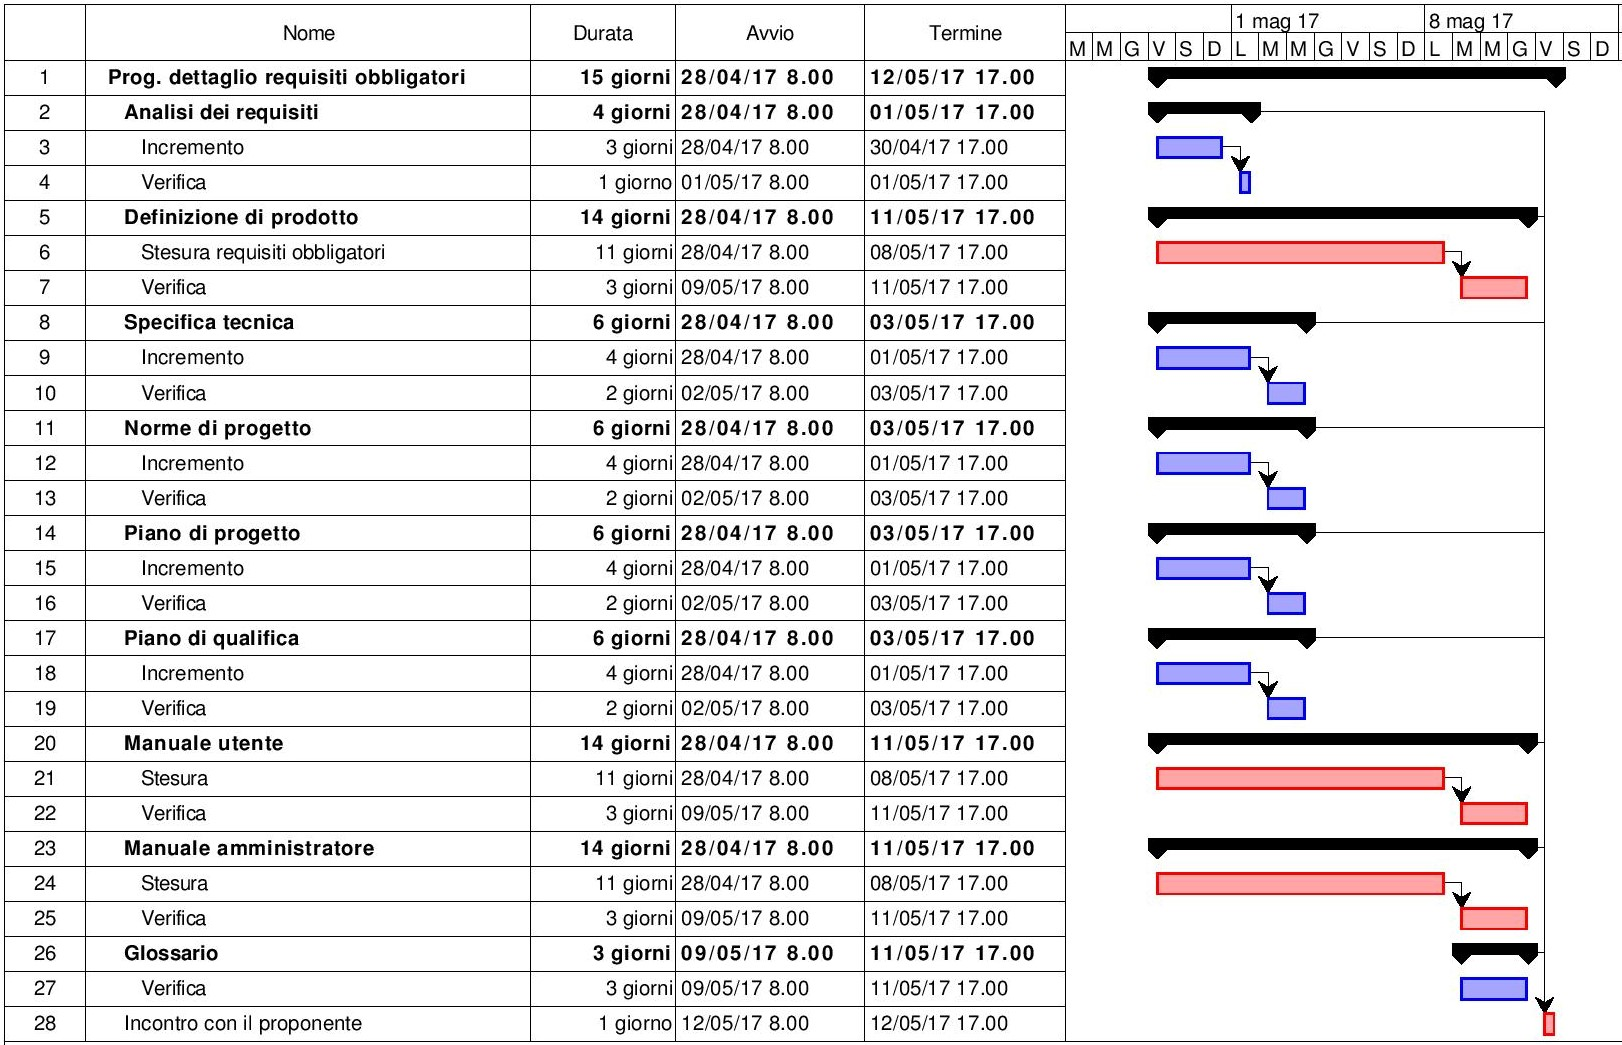
\includegraphics[scale=0.55]{Figures/Gantt_DettaglioObbligatori}
			\caption{Progettazione di dettaglio e Codifica: Diagramma di Gantt}
		\end{figure}
		\begin{figure}[H]
			\centering
			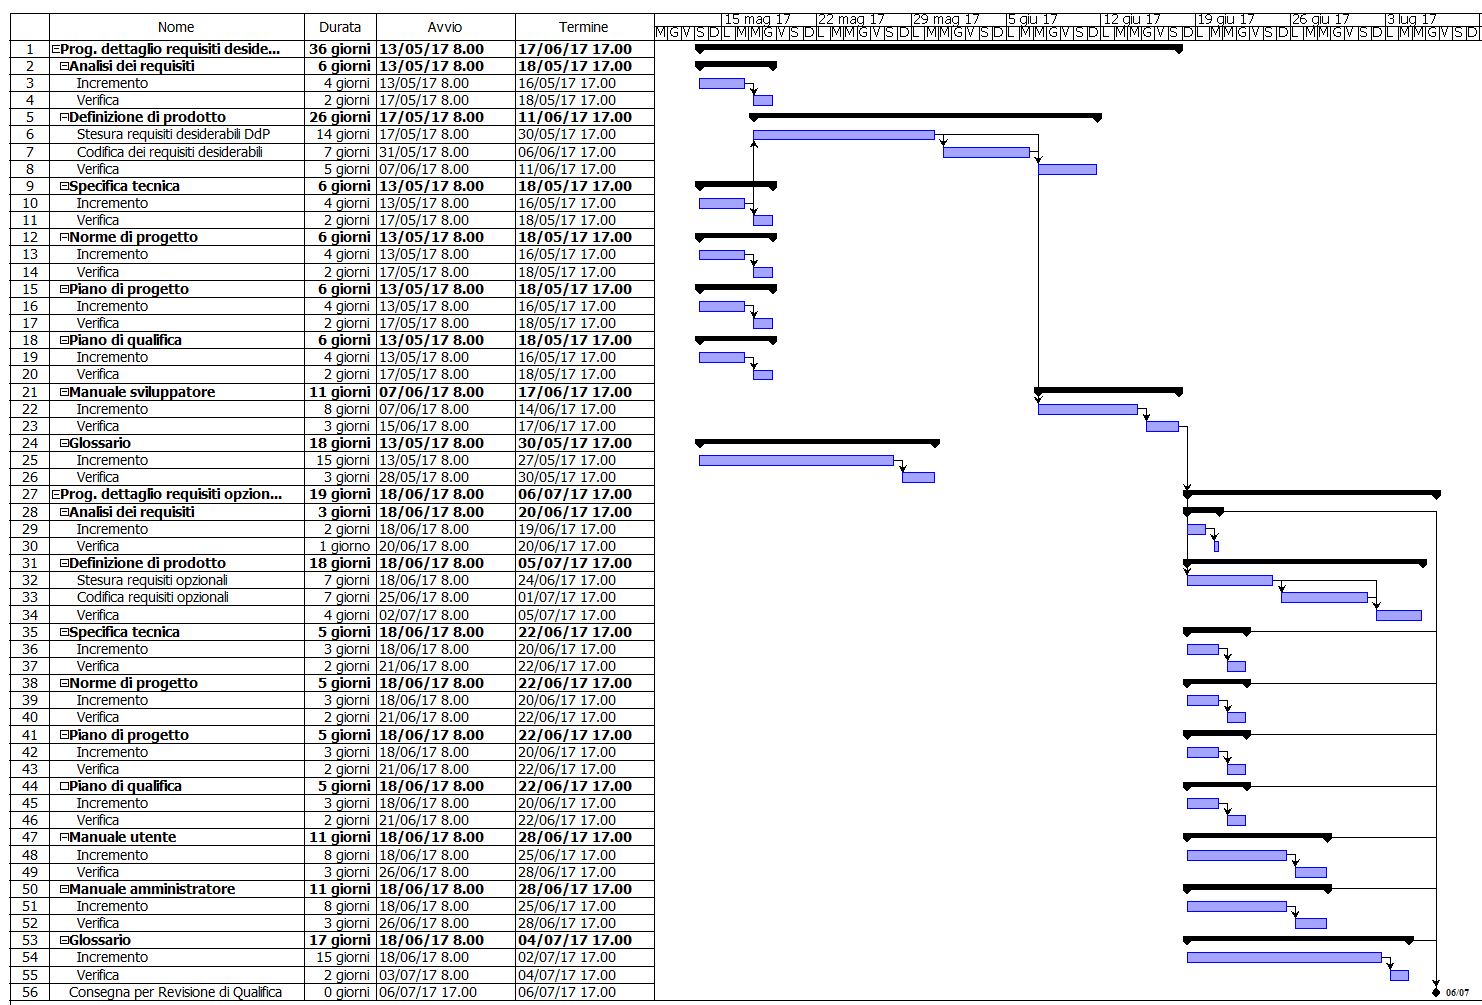
\includegraphics[scale=0.7]{Figures/Gantt_DettaglioOpz}
			\caption{Progettazione di dettaglio e Codifica: Diagramma di Gantt}
		\end{figure}
	
	
		
		\subsection{Validazione}
		\textbf{Periodo} : Da 21/06/2017 a 06/07/2017. \\
		Questo periodo comincia alla fine del periodo di Progettazione di dettaglio e Codifica e prosegue fino alla scadenza della consegna della \revisionediaccettazione.
		\begin{itemize}
			\item \textbf{Validazione}: si controlla che il prodotto soddisfi i requisiti specificati nel documento di \analisideirequisiti ;
			\item \textbf{Collaudo}: il prodotto viene testato in ogni funzionalità richiesta dal capitolato;
			\item \textbf{Incremento e Verifica}:  se necessario vengono aggiornati e verificati i documenti redatti in precedenza, secondo le indicazioni riportate nella valutazione della \revisionediqualifica.
			\item \textbf{Consegna}: il prodotto e i documenti prodotti vengono consegnati al committente durante la \revisionediaccettazione.
		\end{itemize}
		% DIAGRAMMA DI GANTT DELLE ATTIVITÀ
		\begin{figure}[H]
			\centering
			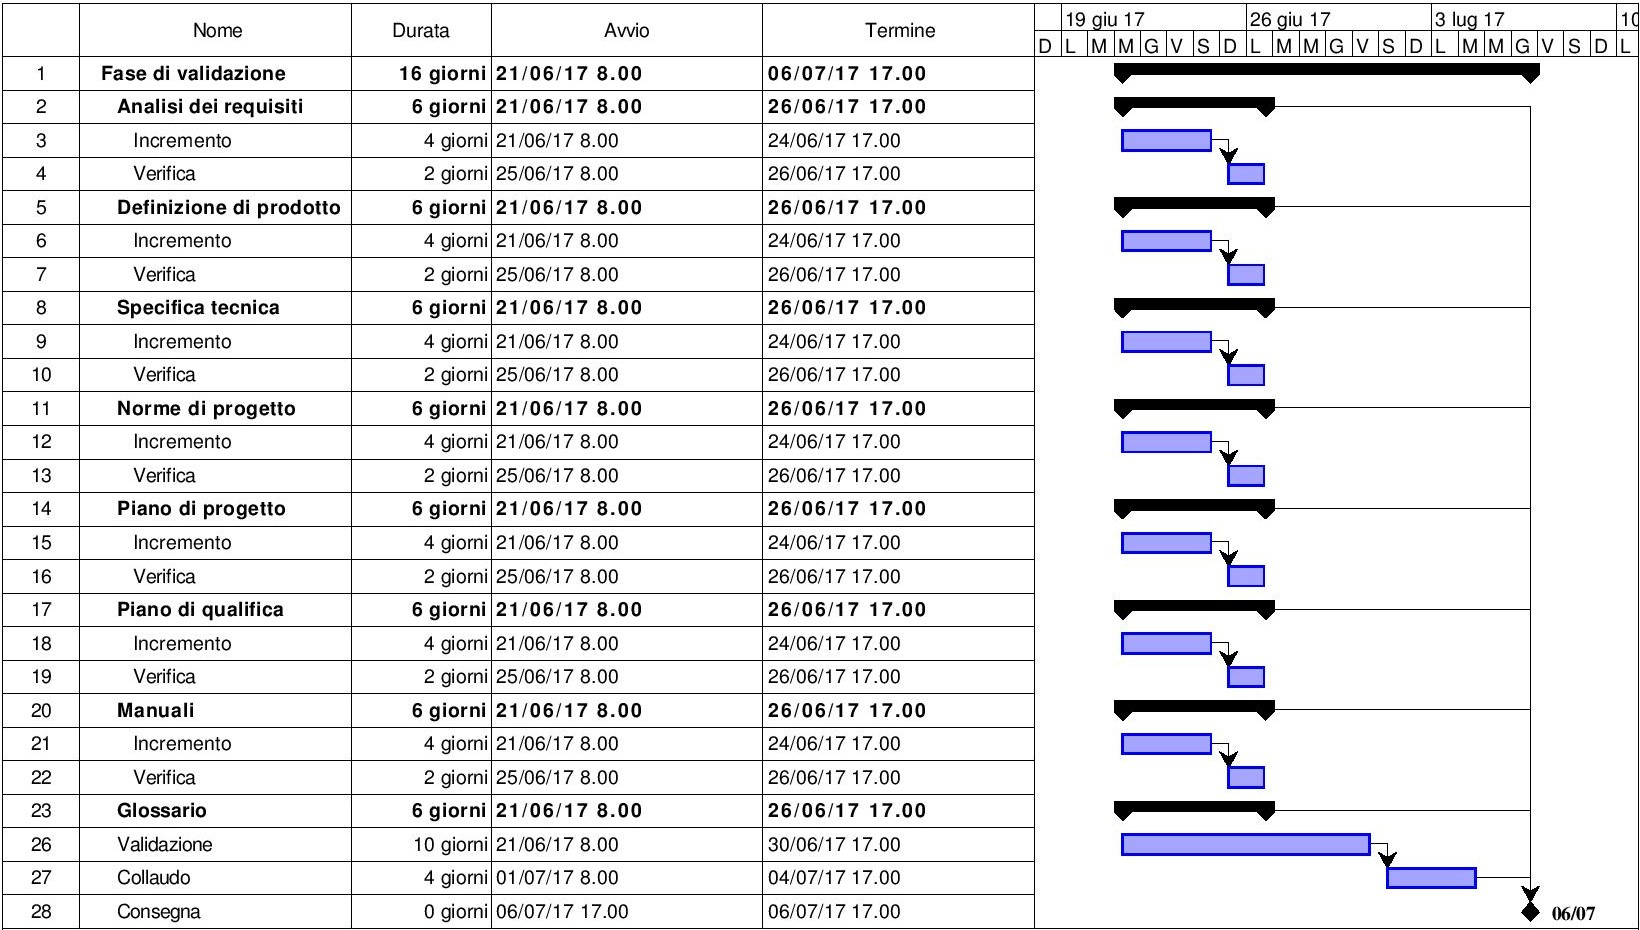
\includegraphics[scale=0.55]{Figures/Gantt_Validazione.jpg}
			\caption{Validazione: Diagramma di Gantt}
		\end{figure}
			
\end{document}
